\section{Příklad 2}
% Jako parametr zadejte skupinu (A-H)
\druhyZadani{H}
\graphicspath{{fig/pr2/}}
\setcounter{figure}{0}

\bigskip


\centerline{\Large{Poďme zjednodušovať!}}
\begin{figure}[H]
\centering
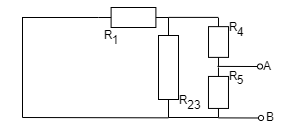
\includegraphics{1.png}
\caption{Odstránime $ R_6 $ a zdroj}
\end{figure}
\begin{figure}[H]
\centering
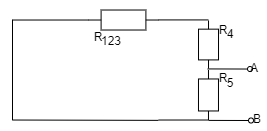
\includegraphics{2.png}
\caption{Spojíme paralelné rezistory $R_1$ a $R_{23}$}
\end{figure}
\begin{figure}[H]
\centering
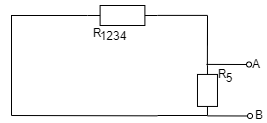
\includegraphics{3.png}
\caption{Spojíme sériové rezistory $R_{123}$ a $R_4$}
\end{figure}\begin{figure}[H]
\centering
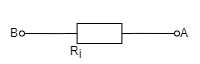
\includegraphics{4.png}
\caption{Máme hľadaný odpor $R_i$}
\end{figure}


\centerline{\Large{Poďme rátať!}}
\centerline{Odpory:}
\bigskip
\centering
\scalebox{1.5}{$R_{23} = R_2 + R_3\hspace{2em}$}
\scalebox{1.5}{$R_{123} = \frac{R_{23} \times R_1}{R_{23} + R_1}\hspace{2em}$}
\scalebox{1.5}{$R_{1234} = R_{123} + R_4\hspace{2em}$}
\\
\medskip
\centering
\scalebox{1.38}{$R_i = \frac{R_{1234} \times R_5}{R_{1234} + R_5} = \frac{(\frac{(R_2 + R_3) \times R_1}{R_2 + R_3 + R_1} + R_4) \times R_5}{\frac{(R_2 + R_3) \times R_1}{R_2 + R_3 + R_1} + R_4 + R_5} = \frac{(\frac{(360 + 580) \times 190}{360 + 580 + 190} + 205) \times 560}{\frac{(360 + 580) \times 190}{360 + 580 + 190} + 205 + 560} = \frac{\num{4 594 800}}{\num{20 861}}\Omega$}
\\
\bigskip
\centerline{A ideme na to:}
\bigskip
\centering
\scalebox{1.45}{$R_{EKV} = \frac{(R_2 + R_3) \times (R_4 + R_5)}{R_2 + R_3 + R_4 + R_5} + R_1 = \frac{(360 + 580) \times (205 + 560)}{360 + 580 + 205 + 560} + 190 = \frac{\num{208 610}}{341}\Omega$}\\
\bigskip
\centering
\scalebox{1.5}{$I = \frac{U}{R_{EKV}} = \frac{220}{\frac{\num{208 610}}{341}} = \frac{\num{7 502}}{\num{20 861}}A$}\\
\bigskip
\scalebox{1.5}{$U_{R_{45}} = U - (I \times R_1) = 220 - (\frac{\num{7 502}}{\num{20 861}} \times 190) = \frac{\num{3 164 040}}{\num{20 861}}V$}\\
\bigskip
\centering
\scalebox{1.5}{$I_{R_{45}} = \frac{U_{R_{45}}}{R_4 + R_5} = \frac{\frac{\num{3 164 040}}{\num{20 861}}}{205 + 560} = \frac{\num{4 136}}{\num{20 861}}A$}\\
\bigskip
\centering
\scalebox{1.5}{$U_i = I_{R_{45}} \times R_5 = \frac{\num{4 136}}{\num{20 861}} \times 560 = \frac{\num{2 316 160}}{\num{20 861}}V$}\\
\bigskip
\centering
\scalebox{1.5}{$I_{R_6} = \frac{U_i}{R_i + R_6} = \frac{\frac{\num{2 316 160}}{\num{20 861}}}{\frac{\num{4 594 800}}{\num{20 861}} + 250} = \frac{\num{231 616}}{\num{981 005}}A \approx \underline{\underline{0.2361A}}$}\\
\bigskip
\centering
\scalebox{1.5}{$U_{R_6} = R_6 \times I_{R_6} = 250 \times \frac{\num{231 616}}{\num{981 005}} = \frac{\num{11 580 800}}{\num{196 201}}V \approx \underline{\underline{59.0252V}}$}
